
\subsection{Experimental Setup}
\subsubsection{Computational Environment}
All experiments were run in Intel Core i5-2310 CPU @ 2.90GHz machines
with 8GB of RAM memory running Linux Mint 13 64 bits.  To facilitate the job distribution we have used the HTCondor framework.

\subsubsection{Parameters}
The GALP algorithm has no settable parameters, the TSLP algorithm on the other hand,
has 3 parameters: the number of iterations of the Tabu Search algorithm (10000),
the size of the tabu list (1000) and the number of random neighbors per iteration
($n_{tabu}$ = 500).
The parameters were set up by empirically experimenting several different combinations.

\subsubsection{Implementation}
To solve the integer programming problems we have used the GLPK LP/MIP solver \cite{GLPK},
version 4.43. We have implemented the heuristics using the Java programming language and
executed/compiled the codes using the Java(TM) SE Runtime Environment (build 1.7.0\_10-b18).
All implementations are available at \url{http://ninfa.inf.ufes.br/ICTAI2013/impl.zip}. 

\subsection{Instance Generator}
To create the instances for our analysis we have implemented a random instance generator.
We have tried to mimic the characteristics of real-world actions supplied by the local EDCO.
Algorithm~\ref{alg:gen} defines the pseudocode of the random instance generator.

\begin{figure}
\begin{algorithm}[H]
\begin{algorithmic}[1]
\Function{Generator}{Correlation factor $\alpha$, Number of years $M$, Number of actions $N$}
\State \label{line:gen1} $BudgetMean \gets Random_{\textit{Uniform}}(700,800)$
\State $BudgetVariance \gets Random_{\textit{Uniform}}(10,20)$
\For{$i=1 \to M$}
  \State $o_{i1} \gets Random_{\textit{Gauss}}(BudgetMean,$ $BudgetVariance)$
\EndFor \label{line:gen2}
\For{$j=1 \to N$}\label{line:gen3}
  \State $c_{j1} \gets \label{line:min} Min(Min(o), Random_{\textit{Uniform}}(1,100))$
\EndFor
\For{$j=1 \to N$}
  \State \label{line:market} $ m_j = 2 Sum(o) / (M \cdot c_{j1})$
\EndFor \label{line:gen4}

\For{$j=1 \to N$} \label{line:W1}
  \For{$i=1 \to M$}
    \State $W_{ji} \gets Random_{\textit{Uniform}}(0,1)$
  \EndFor
  \State $W_{j} \gets ReverSort(W_{j})$
\EndFor

\For{$j=1 \to N$}
  \State $s \gets 0$
  \For{$i=1 \to M$}
    \State $s \gets s + W_{ji}$
  \EndFor
  \For{$i=1 \to M$}
    \State $W_{ji} \gets W_{ji}/s$
  \EndFor
\EndFor  \label{line:W2}

\For{$i=1 \to M$} \label{line:e1}
  \For{$j=1 \to N$}
      \State \label{line:en} $e_{j,k} \gets Max(0, Abs((1-\alpha) \cdot c_{j1} \cdot W_{ji} \, +$
      \State $\qquad \quad \, Random_{\textit{Uniform}}(-100,100) \cdot \alpha))$
  \EndFor
\EndFor \label{line:e2}
\EndFunction
\end{algorithmic}
\caption{Random instance generator}
\label{alg:gen}
\end{algorithm}
\end{figure}

Lines \ref{line:gen1} to \ref{line:gen2} present the generation of the yearly budgets from a Gaussian
distribution (function $GaussRandom(mean, variance)$) that in turn has its variance and mean draw 
from a uniform distribution of fixed parameters (function $URandom(Lower\,bound,\,Upper\,bound)$).
The parameters were inspired by real-world actions, given by the local EDCO.

Lines \ref{line:gen3} to \ref{line:gen4} generate the cost and market of each action, the cost comes from
an uniform random distribution with fixed parameters. Note that in line \ref{line:min} we
use the $Min$ function to guarantee that the action may performed at least one time. Line \ref{line:market}
defines the market of each action as a function of the total budget over all years ($Sum(o)$) and the
cost of the action. That is, the cheapest the action the larger the market.

Lines \ref{line:W1} to \ref{line:W2} are used to build the reverse-ordered normalized weight matrix that is used to 
build the recuperation over the years. After line \ref{line:W2}, the $j$-th line of matrix $W$ will contain
a vector of values that add up to 1 and are reversely ordered, e.g., a possible $W$ matrix for 3 years and 4 actions
could be:
\[ W = \left( \begin{array}{ccc}
0.7 & 0.2 & 0.1 \\
0.8 & 0.1 & 0.1 \\
0.6 & 0.2 & 0.2 \\
1.0 & 0.0 & 0.0 \end{array} \right).\] 

Finally from lines \ref{line:e1} to \ref{line:e2} the electricity recuperation values are defined for each action
and each year. In line \ref{line:en} we may see that the use of matrix $W$ guarantees that the electricity recuperation has a decreasing tendency
over the years. In this line we also present the use of the correlation parameter $\alpha \in [0,1]$.
The closest $\alpha$ is to one, the weaker is the correlation.

The generator was implemented in the Python programming language and its implementation 
and random instances are available at \url{http://ninfa.inf.ufes.br/ICTAI2013/gen.zip}.

\subsection{Time Analysis}

\subsubsection{The Impact of Correlation}                      
It has been demonstrated the classical  Knapsack Problem is pseudo-polynomial
in the size of the input \cite{garey1978} and it is a established
fact that a weak correlation among weight and value greatly reduces the difficulty of the instances \cite{david2005}.
Literature on the knapsack problem states that the difficult problems are the ones that exhibit 
a strong correlation between the value of the item and its weight.

To test if this phenomena also happens in our problem, we have tested the values $[0.0, 0.1, 1.0]$ for $\alpha$,
the parameter that controls the correlation of the value of the action in respect to its cost, 
in a number of problem sizes. When $\alpha$ is 0,
there is a strong correlation between the cost of the action and its electricity return, that is,
the more expensive the action, the more effective it is. When $\alpha$ is 1 there is no correlation
between the value of the actions and its effectiveness. When $\alpha$ is 0.1, there is a weak correlation between cost and value.
The $\alpha$ values of 0.0, 0.1 and 1.0 are equivalent to the following classes of problems defined by \cite{david2005} (respectively): 
\textit{subset sum instances, weakly correlated instances and uncorrelated instances.}

To measure running times we have generated instances for each considered $\alpha$, varying both the amount of years and actions
in the interval $[5,15]$. For each triple defined by the value of $\alpha$, the number of years and actions,
we have generated 10 instances and measured their running time to find the exact solution. 
We have observed that the variance of the running times to solve these 10 instances was too large
for the mean to be significative, so we have adopted a alternative strategy to compare problem sizes
and $\alpha$:
we assume that running times of more than one hour are prohibitive for our application, since
EDCO's usually test several portfolios to make their investment decision. So we consider that
these instances failed to find the solution in practical times.

Figures~\ref{fig:time1} to~\ref{fig:time3} display the amount of instances that successfully executed in less than one hour,
given a value of $\alpha$. For each cell of the figure the exact algorithm was run 10 times using random instances of the problem.
The closer to black, the greater the amount of successful runs. 
From the figures it is clear that the bigger the problem the more likely it is that it will take more than one hour to execute, 
since cells closer to $(15,15)$ tend to be closer to white.
Also, it may be observed that the more
correlated the cost is with the profit (the smaller the $\alpha$),
the harder the problems seems to be, as predicted by the literature.

%\begin{subfigure}[b]{0.3\textwidth}
%  \includegraphics[width=\textwidth]{mouse}
%  \caption{A mouse}
%  \label{fig:mouse}
%\end{subfigure}

\begin{figure}
  \begin{subfigure}{0.45\textwidth}
    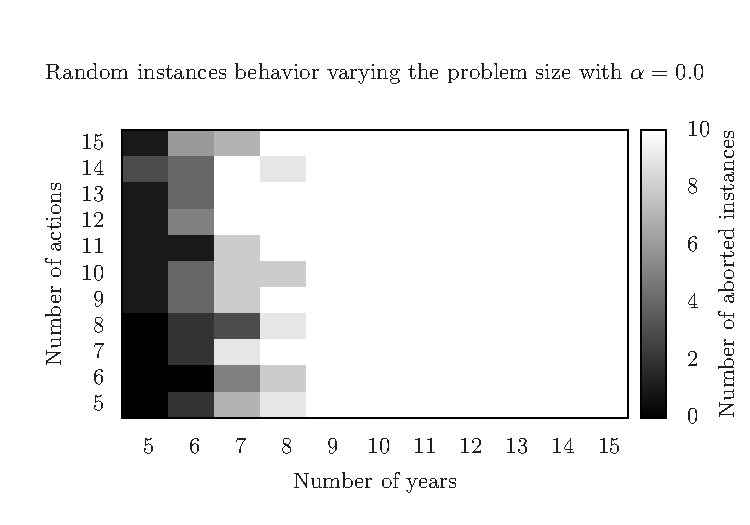
\includegraphics[scale=0.5, trim=0.75cm 0cm 0 2cm, clip=true]{imgs/very_hard.pdf}
    \caption{Strong correlation between cost and profit.}
    \label{fig:time1}
  \end{subfigure}
  \qquad
  \begin{subfigure}{0.45\textwidth}
    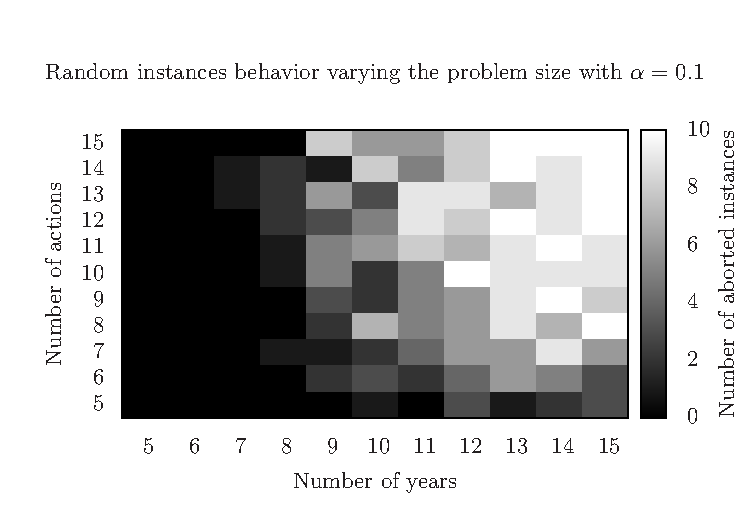
\includegraphics[scale=0.5, trim=0.75cm 0cm 0 2cm, clip=true]{imgs/hard.pdf}
    \caption{Weak correlation between cost and profit. \\ $\,$ }
    \label{fig:time2}
  \end{subfigure}
\end{figure}

%\begin{subfigure}
%  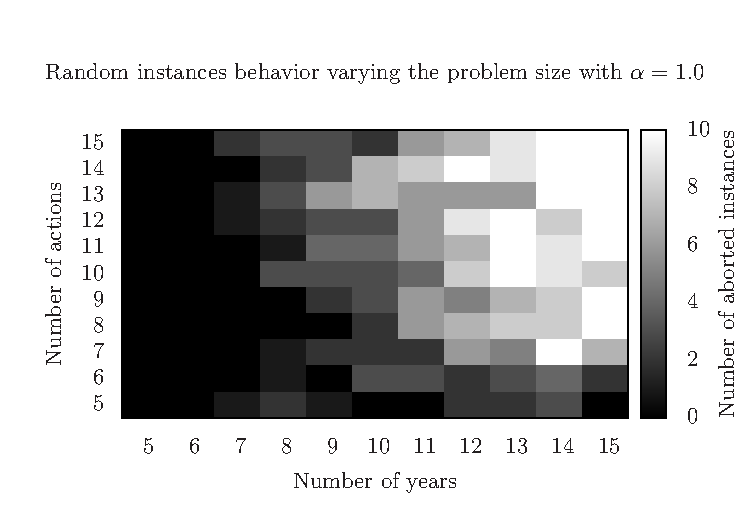
\includegraphics[scale=0.5, trim=0.75cm 0cm 0 2cm, clip=true]{imgs/easy.pdf}
%  \caption{No correlation between cost and profit.}
%  \label{fig:time3}
%\end{subfigure}


\subsection{Solution Analysis - Easy Instances}

In this subsection we compare the solution quality of the implemented heuristics
in the set of easy instances, there is, the instances in which the exact algorithm
found the optimal solution in less than one hour. We have also limited the running time
of the heuristics in one hour.

Figures~\ref{fig:mh1_1} to \ref{fig:mh2_3} display the average ratio between the optimal solution (when available) 
and the solution found by the heuristics. 
Small relative ratios are darker than large differences.
A ratio of 1 means that the heuristic has found a solution with the same quality
than the exact algorithm.
When no solution was found by the exact approach in less than one hour for 
a tripe $(\alpha, years, actions)$, we display the value ``$na$'' in
the corresponding cell.

Figures~\ref{fig:mh1_1} to \ref{fig:mh2_3} show that all heuristics managed
to find very close solutions to the exact (less than 1\% difference).
Also, the paler aspect of the TSLP figures (specially when $\alpha=0.0$) suggests that
it managed to beat the GALP algorithm considering solution quality.
In fact, considering only these easier problem sizes, the paired Wilcoxon signed-rank test \cite{japkowicz2011evaluating} rejects the null hypothesis
that the algorithms are the same with a $p$-value of less than $10^{-11}$.

\begin{figure}
\centering
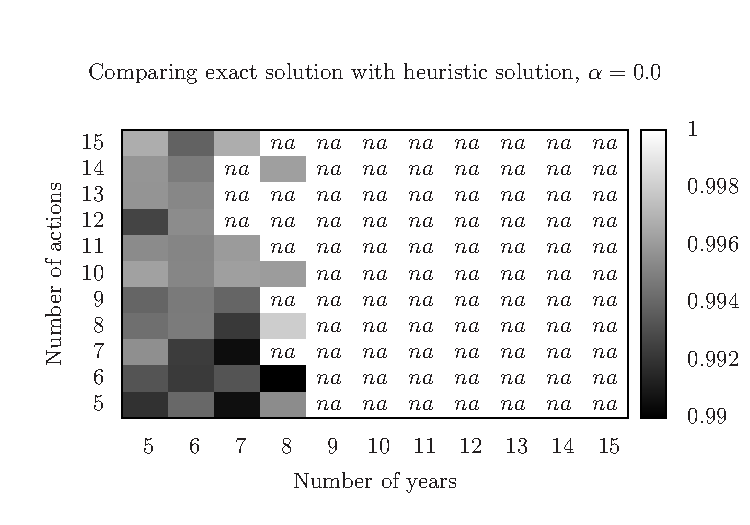
\includegraphics[scale=0.5, trim=0.75cm 0cm 0 2cm, clip=true]{imgs/comp_very_hard.pdf}
\caption{Comparison between the optimal solution (when available) 
and the solution by the GALP for $\alpha=0.0$.}
\label{fig:mh1_1}
\end{figure}

\begin{figure}
\centering
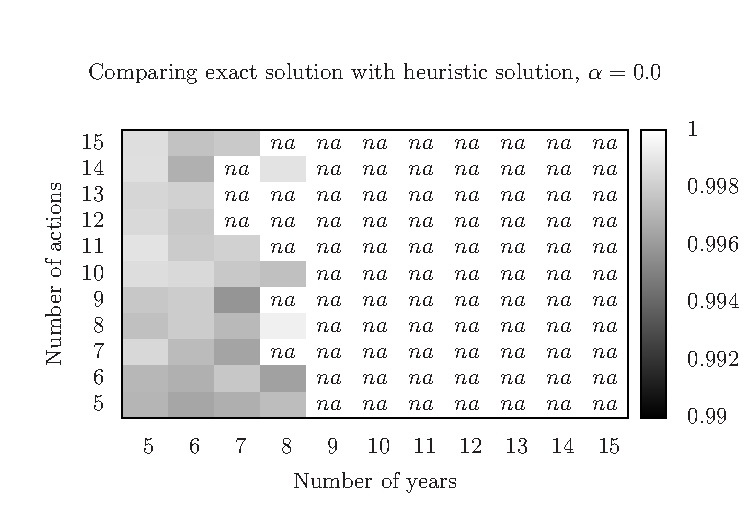
\includegraphics[scale=0.5, trim=0.75cm 0cm 0 2cm, clip=true]{imgs/comp_very_hard_ts.pdf}
\caption{Comparison between the optimal solution (when available) 
and the solution by the TSLP for $\alpha=0.0$.}
\label{fig:mh2_1}
\end{figure} 

\begin{figure}
\centering
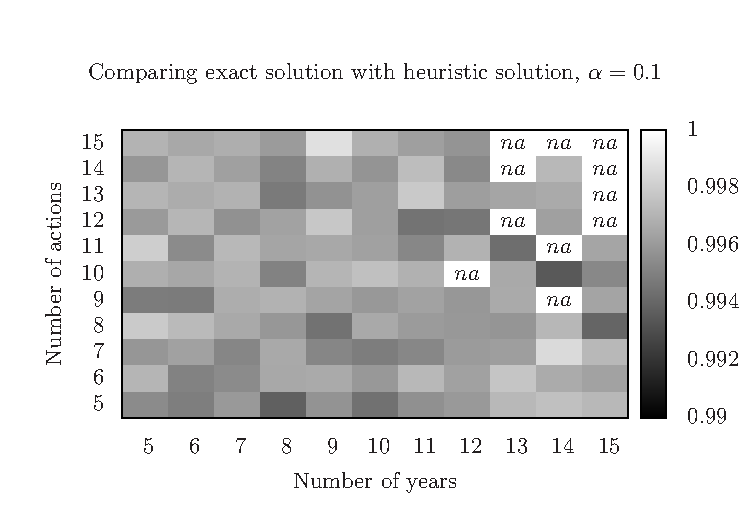
\includegraphics[scale=0.5, trim=0.75cm 0cm 0 2cm, clip=true]{imgs/comp_hard.pdf}
\caption{Comparison between the optimal solution (when available) 
and the solution by the GALP for $\alpha=0.1$.}
\label{fig:mh1_2}
\end{figure}

\begin{figure}
\centering
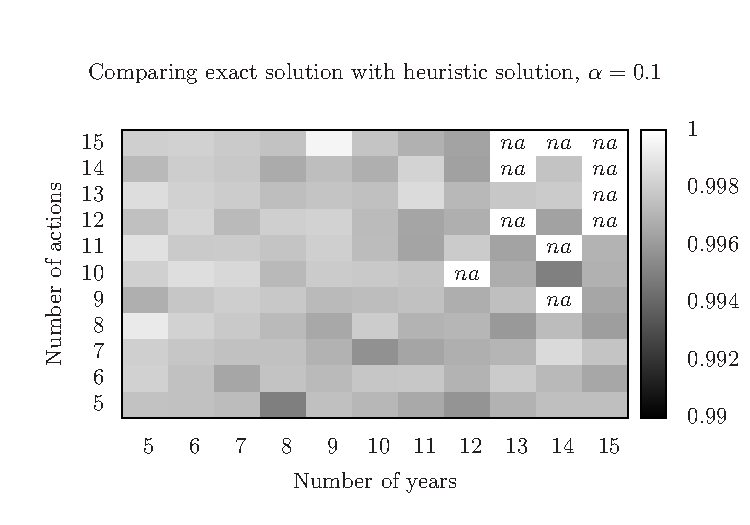
\includegraphics[scale=0.5, trim=0.75cm 0cm 0 2cm, clip=true]{imgs/comp_hard_ts.pdf}
\caption{Comparison between the optimal solution (when available) 
and the solution by the TSLP for $\alpha=0.1$.}
\label{fig:mh2_2}
\end{figure}
 
\begin{figure}
\centering
%\vspace{1mm}
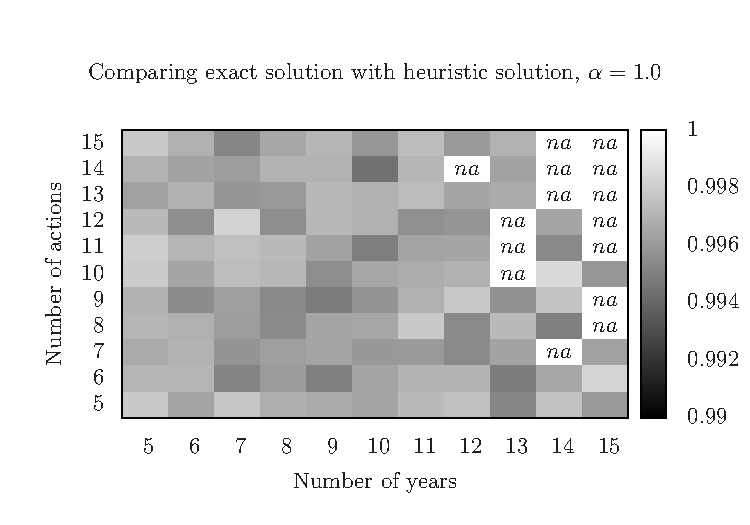
\includegraphics[scale=0.5, trim=0.75cm 0cm 0 2cm, clip=true]{imgs/comp_easy.pdf}
\caption{Comparison between the optimal solution (when available) 
and the solution by the GALP for $\alpha=1.0$.}
\label{fig:mh1_3}
\end{figure}

\begin{figure}
\centering
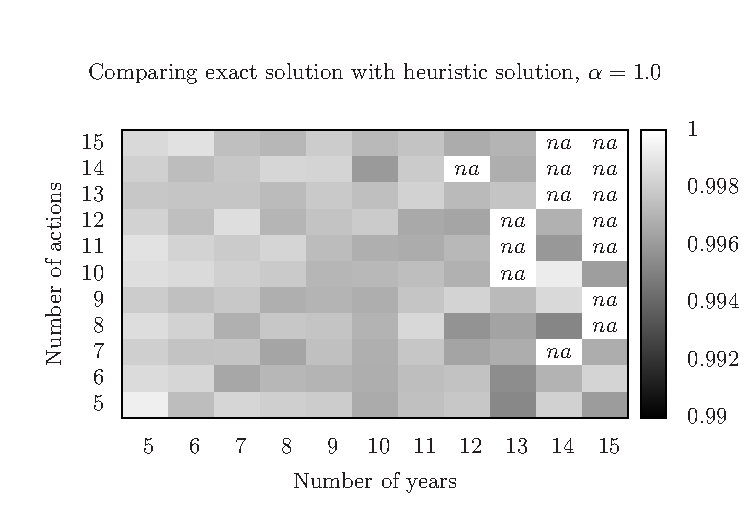
\includegraphics[scale=0.5, trim=0.75cm 0cm 0 2cm, clip=true]{imgs/comp_easy_ts.pdf}
\caption{Comparison between the optimal solution (when available) 
and the solution by the TSLP for $\alpha=1.0$.}
\label{fig:mh2_3}
\end{figure}


\subsection{Solution Analysis - All Instances}

In this subsection we compare the behavior of the metaheuristics in respect to one another
considering all instances. We cannot compare the results with the optimal solution since they are unknown for the harder instances.

Figures~\ref{fig:comp_1} to \ref{fig:comp_3} display the relative distance between the two proposed 
heuristics considering the solution quality for the three studied correlation values.
Each cell contains the mean ratio between the quality of the GAPL and TSLP algorithms,
here the mean is meaningful because the values of the ratio have a reasonable variance.

From the scale of the figures (varying between 1 and 0.993 at most) it is clear
that both algorithms achieved very similar results, however the TSLP algorithm
managed to outperform the GAPL, in average, in every cell of the figures (no value is greater than 1).
However GALP did manage to outperform the TSLP algorithm in some instances of the problem,
so we perform the paired Wilcoxon signed-rank to confirm that the TSLP is indeed superior
to the GALP algorithm. And again we may reject that null hypothesis that the algorithm
are equal with a $p$-value of less than $10^{-11}$.

\begin{figure}
\centering
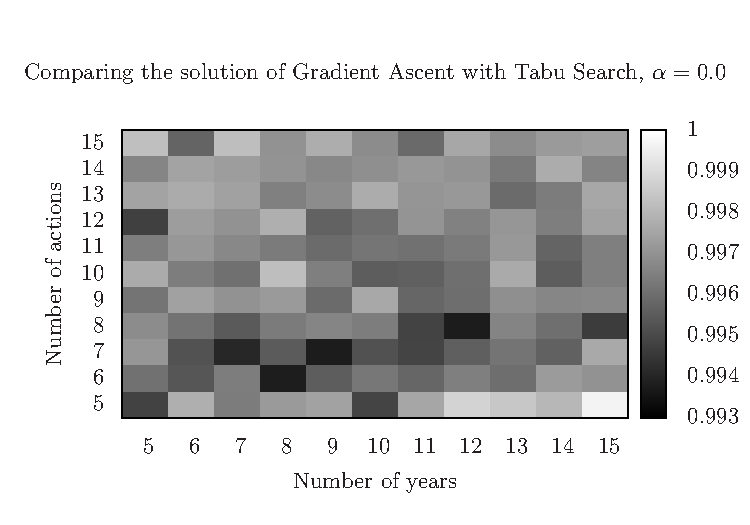
\includegraphics[scale=0.5, trim=0.75cm 0cm 0 2cm, clip=true]{imgs/comp_very_hard_sg_ts.pdf}
\caption{Relative distance between the two proposed heuristics for $\alpha=0.0$.}
\label{fig:comp_1}
\end{figure}


\begin{figure}
\centering
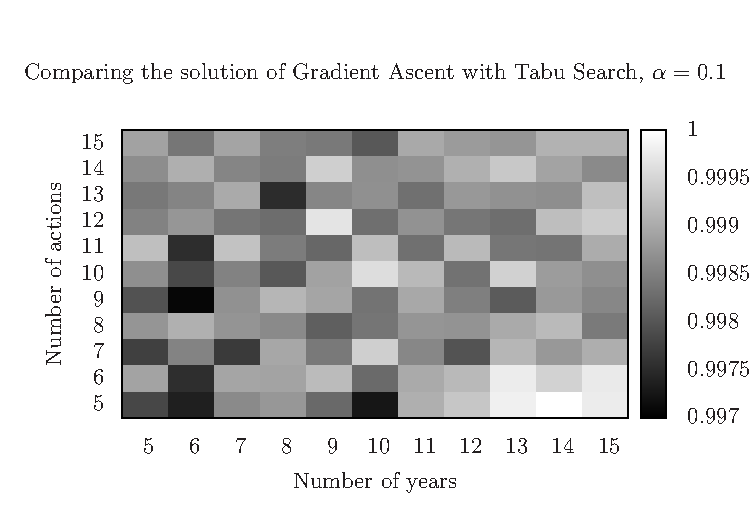
\includegraphics[scale=0.5, trim=0.75cm 0cm 0 2cm, clip=true]{imgs/comp_hard_sg_ts.pdf}
\caption{Relative distance between the two proposed heuristics for $\alpha=0.1$.}
\label{fig:comp_2}
\end{figure}

\begin{figure}
\centering
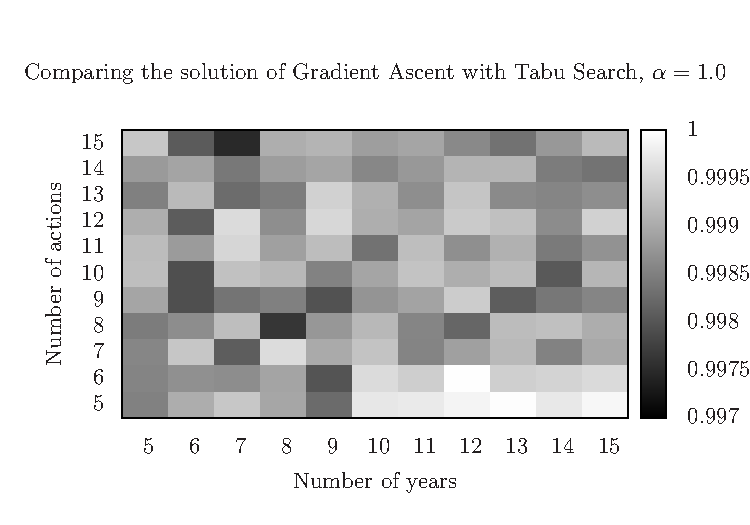
\includegraphics[scale=0.5, trim=0.75cm 0cm 0 2cm, clip=true]{imgs/comp_easy_sg_ts.pdf}
\caption{Relative distance between the two proposed heuristics for $\alpha=1.0$.}
\label{fig:comp_3}
\end{figure}

Figures~\ref{fig:lpgavsmip} and \ref{fig:lptsvsmip} display the histogram of
the ratio of the solution found by the heuristic algorithms and the optimal solution.
From the histograms we can conclude that TSLP has a better behavior than GALP,
showing a smaller variance and larger ratio mean.

Although the time limit was set to one hour, the TSLP had a maximum running time of less than one minute, with an average time of 20 seconds, and GALP had a negligible running time for all instances.

\begin{figure}
\centering
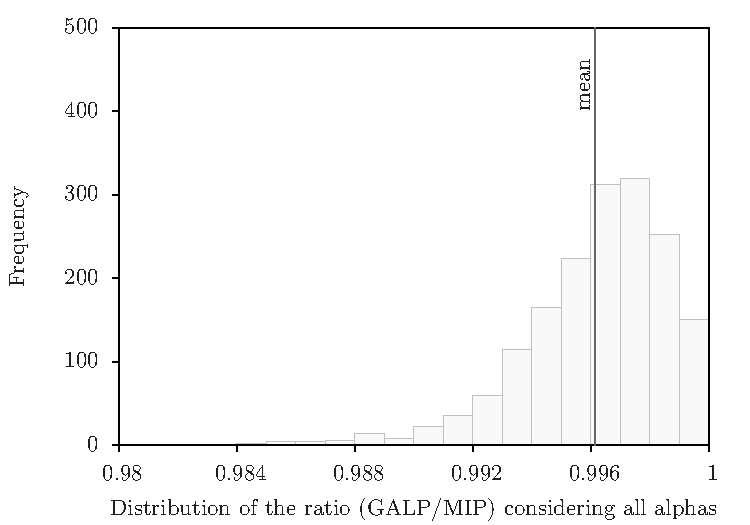
\includegraphics[scale=0.7, trim=1cm 0 0 0]{imgs/lpgavsmip.pdf}
\caption{Histogram of the ratio of the solution found by the GALP heuristic and the optimal solution.}
\label{fig:lpgavsmip}
\end{figure}

\begin{figure}
\centering
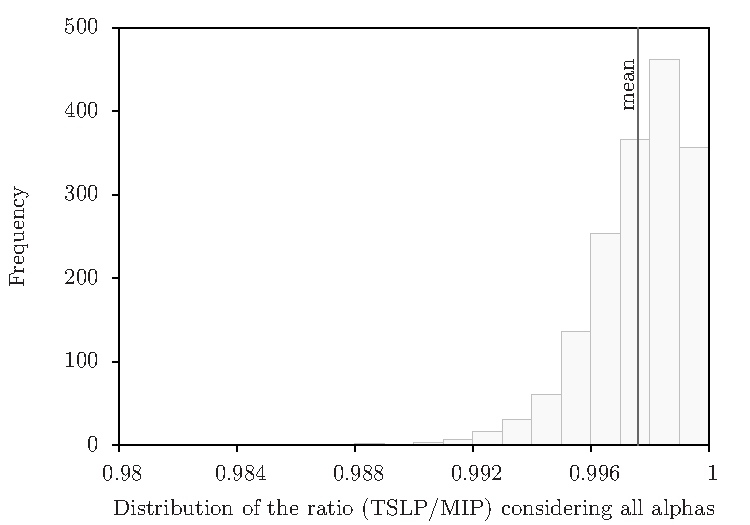
\includegraphics[scale=0.7, trim=1cm 0 0 0]{imgs/lptsvsmip.pdf}
\caption{Histogram of the ratio of the solution found by the TSLP heuristic and the optimal solution.}
\label{fig:lptsvsmip}
\end{figure}

% From the figures it is clear that the TSLP algorithm is superior

